\documentclass[12pt,a4paper]{article}

% for figures
\usepackage{graphicx}

% for subfigure
\usepackage{caption} % for subfigure
\usepackage{subcaption}  % for subfigure





\begin{document}

The person in Fig. \ref{albert} is Albert.





% ONE FIGURES
\begin{figure}
	
\includegraphics[height=50mm]{albert.jpg}
	\caption{This is Albert.} \label{albert}
\end{figure}





% TWO FIGURES
\begin{figure}
	\centering
	
\includegraphics[height=50mm]{albert.jpg}
	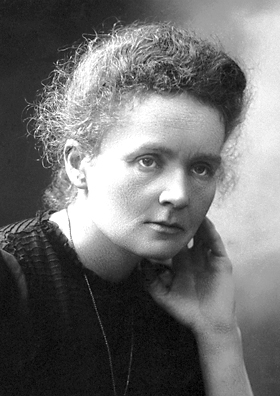
\includegraphics[height=50mm]{curie.jpg}
	\caption{This is Albert and Curie.} \label{albert2}
\end{figure}





% SUBFIGURE
\begin{figure}
	\centering

	\begin{subfigure}[h]{6cm}
		
\includegraphics[width=5 cm]{albert.jpg}
		\caption{This is also Albert.} \label{sub21}
	\end{subfigure}
	~ % to get side-by-side
	\begin{subfigure}[h]{6cm}
		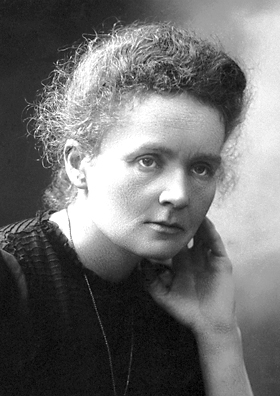
\includegraphics[height=60mm]{curie.jpg}
		\caption{This is Curie.} \label{sub22}
	\end{subfigure}
	
	\caption{This is both.} \label{fig2}

\end{figure}





% MINIPAGE
\begin{figure}
	\centering

	\begin{minipage}[h!]{3cm}
		\centering
		
\includegraphics[height=3cm]{albert.jpg}
		\caption{This is also Albert with minipage.} \label{sub31}
	\end{minipage}

	\begin{minipage}[h!]{3cm}
		\centering
		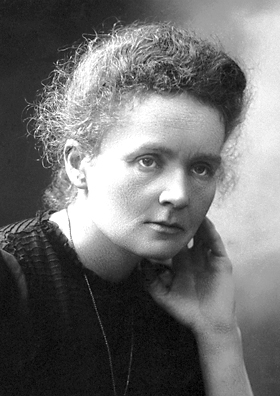
\includegraphics[height=30mm]{curie.jpg}
		\caption{This is Curie with minipage.} \label{sub32}
	\end{minipage}
	
	\caption{This is both with minipage.} \label{fig3}

\end{figure}





% MINIPAGE
\begin{figure}
	\centering

	\begin{minipage}[h!]{5cm}
		\centering
		
\includegraphics[width=3cm]{albert.jpg}
		\caption{This is also Albert with minipage.} \label{sub41}
	\end{minipage}

	\begin{minipage}[h!]{5cm}
		\centering
		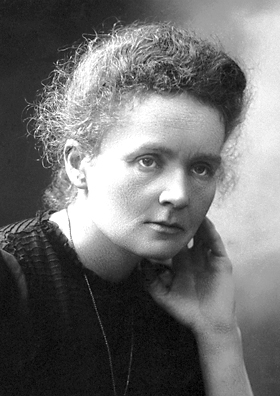
\includegraphics[height=30mm]{curie.jpg}
		\caption{This is Curie with minipage.} \label{sub42}
	\end{minipage}
	
	\caption{This is both with minipage.} \label{fig4}

\end{figure}




\end{document}